\documentclass[12pt]{amsart}

% \usepackage{ucs}
% \usepackage[utf8x]{inputenc}
\usepackage{amsmath}
\usepackage{amsfonts}
\usepackage{amssymb}
\usepackage{amsthm}
% \usepackage{babel}
\usepackage{fontenc}
\usepackage{graphicx}

\usepackage[usenames,dvipsnames]{xcolor}
\usepackage{hyperref}

\hypersetup{%
  colorlinks=false,% hyperlinks will be black
  urlbordercolor= OliveGreen,% hyperlink borders will be red
  pdfborderstyle={/S/U/W 1}% border style will be underline of width 1pt
}

\usepackage{setspace}
\usepackage[margin=1in]{geometry}
\usepackage{listings}
% \date{July 2014}
\usepackage{paralist}
\usepackage{tikz}
%opening
\title{Semantic enrichment of mathematics \\ for accessibility and display on 
the web}
\author{Volker Sorge, Davide Cervone, Peter Krautzberger}



% \makeatletter
% 
% \def\section{\@startsection{section}{1}\z@
%     \z@% Vertical space before heading
%     {1sp}% Space after heading (if <= 0, heading is inlined)
%   {\normalfont\scshape\centering}}
% 
% \def\subsection{\@startsection{subsection}{2}\z@
%     \z@{-.5em}%
%   {\normalfont\bfseries}}
% 
% \def\subsubsection{\@startsection{subsubsection}{3}%
%   {\parindent}\z@{-.5em}%
%   {\normalfont\itshape}}
% 
% \def\maketitle{\par
%   \@topnum\z@ % this prevents figures from falling at the top of page 1
%   \thispagestyle{empty}% this sets first page specifications
%   \uppercasenonmath\shorttitle
%   \ifx\@empty\shortauthors \let\shortauthors\shorttitle
%   \else \andify\shortauthors
%   \fi
%   \@maketitle@hook
%   \begingroup
%       \toks@\@xp{\shortauthors}\@temptokena\@xp{\shorttitle}%
%       \toks4{\def\\{ \ignorespaces}}% defend against questionable usage
%       \edef\@tempa{%
%         \@nx\markboth{\the\toks4
%           \@nx\MakeUppercase{\the\toks@}}{\the\@temptokena}}%
%       \@tempa
%   \endgroup
%     \begingroup
%         \@maketitle
%     \endgroup
%   \c@footnote\z@
%   \@cleartopmattertags
% }
% 
% \def\@maketitle{%
%   \normalfont\normalsize
%   \@adminfootnotes
%   \global\topskip\z@% 42\p@\relax % 5.5pc   "   "   "     "     "
%   \@settitle
%   \ifx\@empty\authors \else \@setauthors \fi
%   \normalsize
%   \if@titlepage
%     \newpage
%   \else
%     % \dimen@34\p@ \advance\dimen@-\baselineskip
%     % \vskip\dimen@\relax
%   \fi
% } % end \@maketitle
% 
% \def\@setauthors{%
%   \begingroup
%   \def\thanks{\protect\thanks@warning}%
%   \trivlist
%   \centering\footnotesize \@topsep0\p@\relax
%   \advance\@topsep by -\baselineskip
%   \item\relax
%   \author@andify\authors
%   \def\\{\protect\linebreak}%
%   \MakeUppercase{\authors}%
%   \ifx\@empty\contribs
%   \else
%     ,\penalty-3 \space \@setcontribs
%     % too late to close toccontribs, the .itd file has
%     % already been written.
%     % \@closetoccontribs
%   \fi
%   \endtrivlist
%   \endgroup
% }
% 
% \def\@settitle{\begin{center}%
%   \baselineskip15\p@\relax
%     \bfseries
% \uppercasenonmath\@title
%   \@title
%   \end{center}%
% }
% \makeatother

\begin{document}
\doublespacing
\maketitle


We propose to develop and integrate heuristics for semantic enrichment of MathML 
into MathJax, the open-source JavaScript display engine for mathematics. The 
enrichment will be applied to solve two major problems for mathematics on the 
web: ubiquitous math accessibility, and responsive rendering of equations. The 
proposed work is based on our existing and reliable open-source technology, which 
has been developed for over 5 years and is deployed across the scientific, 
educational, and industrial ecosystem on the web.

\section{Mathematics and the Open Web Platform}

Mathematical notation is a core component of educational, scientific, and 
industrial communication. It provides a universal method to communicate complex 
ideas in a precise form, balancing the flexibility to develop new forms of 
expression with a rigor to remain accessible. The World Wide Web Consortium's 
(W3C) \href{https://en.wikipedia.org/wiki/Open_Web_Platform}{Open Web Platform} 
is the most important communication platform today and it is rapidly becoming 
the dominating publishing platform. Despite the many advances in
browser and web-authoring technologies, however, 
scientific content on the web frequently still is forced 
into static images. 

Mathematics plays a vital role in emerging web standards as the only field with 
a W3C specification -- \href{http://www.w3.org/Math/draft-spec/}{MathML}. Today, 
MathML is the primary format for mathematical content, in 
particular in publishing workflows. While authors favor a variety of options 
such as equation editors and \LaTeX, conversion to MathML is commonplace.

\subsubsection*{Semantic enrichment}

Despite its success, MathML currently is used more for output than
exchange.  One might compare this to the situation with graphics
formats, where JPG and PNG are good for output, but SVG is a better
format for exchange of graphical data.

MathML comes in two flavors: Presentation MathML and 
Content MathML. Presentation MathML is geared towards visual display, playing a 
role similar to Microsoft Office XML and \LaTeX\ for print. It provides common 
layout elements (sub-/superscripts, fractions, roots, etc.), styles, and 
attributes. While it is sufficient to lay out mathematics, expressions usually 
do not exhibit enough structure to infer meaning.

In contrast, Content MathML aims to serve as a semantic exchange format for 
mathematical software systems. It provides elements with relatively precise 
mathematical semantics (divide, interval, matrix, etc.)~leading to 
representations inspired by mathematical logic (e.g., lambda 
calculus). Thus, while Content MathML is suitable for conveying semantics 
between systems, it does not lend itself to a human-oriented style, which often 
mixes semantic with presentational elements. This limitation also shows in the 
lack of authoring tools and existing content repositories for Content MathML.

The dominance of Presentation MathML combined with the shortcomings of Content 
MathML severely limit the use and re-use of MathML content, as it adds 
significant complexity for any  technology that digests MathML, in particular for
accessibility (e.g., voicing, navigation), search, and scientific computing. 

Real-world mathematics mixes semantics and presentation to enhance both. A 
successful exchange of MathML, therefore, depends on pragmatic solutions within the 
existing ecosystem. This means building on Presentation MathML instead of 
overly abstract Content MathML, with openly documented and extensible APIs to 
enrich expressions.

We propose to develop an open-source JavaScript solution as part of the MathJax 
project to help solve this problem. It will provide an implementation of 
heuristics and APIs to create semantically enriched MathML from \TeX, Asciimath, 
and MathML. We will use this to build solutions for two major problems for 
mathematical content on the web today: ubiquitous accessibility, and rendering 
on mobile devices.


\subsubsection*{Accessibility}

Ensuring accessibility to scientific material has always been a challenging 
task and a major obstacle for full inclusiveness in education in the 
traditional STEM subjects (science, technology, engineering, and mathematics), 
in particular at the late secondary and tertiary stages. As teaching moves 
towards the web, we are faced with rapidly changing content, employing media 
ranging from traditional articles containing mathematical formulas and 
scientific diagrams to highly interactive web pages with dynamic diagrams or 
simulations.  This makes traditional approaches to accessibility all but obsolete. 

In addition, accessibility goes beyond the traditional ideas of aural
rendering and magnification that make content 
accessible for users who are visually impaired or deaf. It also includes 
support for those with cognitive impairments or learning disabilities, who
often need solutions such as 
highlighting, changes in contrast, or spatial re-representation.

The Open Web Platform holds the promise of greatly enhancing accessibility. 
Still, the reliance on expensive, specialist software creates an even higher 
obstacle for inclusive education. To make matters worse, users and publishers 
currently are left without a reliable solution for mathematics on the open web.

We will leverage the semantically enriched MathML to generate speech text (e.g. 
``f of x equals x squared''), enable exploration of mathematical expressions, 
and provide APIs for accessibility tools like screenreaders. Incorporating 
accessibility directly into the MathJax core will provide a ubiquitous 
accessibility solution on all browsers and platforms.

\subsubsection*{Responsive equations.}

Rendering equations on mobile devices is extremely challenging: they often 
fail to reflow or become illegible through iterated line-breaks. We will 
use the semantic enrichment to develop a novel rendering for small screens by 
re-arranging and collapsing subexpressions. This will present an ``outline'' to the 
reader that fits faithfully on the screen while providing the means to navigate 
and explore and expand the expression further.

\subsubsection*{Future continuation.} We hope to significanly advance this 
work in all three aspects in a second development year as described in the 
appendix.

\section{Prior Work}

\subsubsection*{MathML authoring and conversion}

A key problem of MathML is the lack of good authoring solutions. In fact, 
MathML is rarely used as a direct authoring format. Instead, authors use tools 
with custom formats such as graphical equation editors, \TeX/\LaTeX, or computing 
software. This diversity is desirable so that authors can find solutions that 
fit their needs.

While some tools export to MathML, others (notably  \LaTeX) do not. This leads 
to an ecosystem of conversion tools of varying output quality. In either case, 
the resulting markup is usually limited to Presentation MathML. 
Similarly, enriching MathML will happen during import into an internal format.

\subsubsection*{Accessibility}

Until 2013, the only MathML accessibility solution was 
\href{http://www.dessci.com/en/products/mathplayer/}{MathPlayer}, available as 
a plugin for Internet Explorer. Unfortunately, Microsoft abandoned support for 
plugins like MathPlayer starting with Internet Explorer 10. In 2013, Google's 
screen reader, \href{http://www.chromevox.com/}{ChromeVox}, gained MathML 
support. In late 2013, 
\href{http://www.apple.com/accessibility/}{Apple VoiceOver}
incorporated rudimentary MathML support.

MathPlayer and ChromeVox apply heuristics to generate a semantic structure from 
Presentation MathML and use this to voice and navigate equations. While MathPlayer is the 
gold standard, it is proprietary, undocumented, and now effectively unavailable.

\subsubsection*{MathJax and ChromeVox}

Our proposal's main focus is the open-source 
\href{http://www.mathjax.org}{MathJax project}, a joint venture 
of the American Mathematical Society and the Society for Industrial and Applied 
Mathematics. Founded in 2008, MathJax solves the chicken-and-egg problem of 
MathML: no browser support $\Rightarrow$ no published MathML $\Rightarrow$ no 
browser support $\Rightarrow$ \ldots 

MathJax is centered around its eponymous JavaScript library for rendering 
mathematics. It is  a highly modular, input- and output-agnostic display engine 
that ``just works''. Today, MathJax is the default solution for math on the web 
thanks to universal browser support, a large test suite, and a rich API. It is 
also used in desktop and mobile applications and the free MathJax CDN service 
has grown to ~100 million unique visitors per month.

While MathJax is known for ease-of-use and visual quality, it was designed with 
accessibility in mind. This includes a user interface for magnification and 
copy\&paste, as well as smooth interaction with MathPlayer and ChromeVox. In 
2013, the MathJax and ChromeVox teams collaborated to enhance ChromeVox's 
voicing and navigation of MathJax output. This collaboration will find a 
continuation in a joint project with Benetech in August 2014 to provide 
server-side, accessible SVG image rendering for non-JavaScript environments.

In the project proposed here, we will combine our expertise with mathematical rendering and 
accessibility to extend MathJax to ubiquitous enrichment, accessibility, and 
responsive rendering of mathematics.


\section{Research Approach}

We will develop JavaScript applications to generate semantically enriched  
MathML as well as two rendering tools to leverage this enrichment. To 
summarize we propose to build

\begin{compactenum}
\item an application implementing heuristic algorithms to process 
MathML and embed semantic information in the original MathML,
\item an application that creates  and embeds speech-strings in MathML for 
voicing, navigation, and synchronized highlighting by screenreaders, and,
\item an application for ``responsive equations'', i.e., meaningful rendering 
on mobile 
devices by re-arranging and collapsing content as well as a user 
interface for exploration.
\end{compactenum}

\subsection{Semantic enrichment}

For semantic enrichment we decided against Content MathML, as it is 
impractical for in human-oriented presentation. We therefore propose 
to adapt and improve an approach used by the ChromeVox screen reader. It is based on 
the heuristic interpretation of Presentation MathML into a custom semantic 
representation that is modeled on 
\href{http://en.wikipedia.org/wiki/K-16_(education)}{K-16} mathematics.

The main problem for semantic enrichment of Presentation MathML is to transform 
its flat structure into one that correctly determines the scope of operators, 
relations, etc.  Our approach aims to represent a formula in a semantic tree 
structure akin to a term tree. The semantic tree is assembled bottom-up, where 
we first classify the single components of an expression, giving each an 
immutable type and a mutable role. The former aims to capture the basic nature 
of the symbol, while the latter is used to describe the role of a symbol in the 
context of the formula. For example, $f$, which has the type ``Latin letter'' 
can have the role of an identifier in $f + g$ but that of a function in 
$f(x)$.

A central heuristic then builds term trees from flat structures by promoting 
relations and defining operator precedence orders as well as determining 
properly delimited structures. As an example of this heuristic we observe how 
the quadratic formula is rewritten from its Presentation MathML representation 
into its semantic interpretation below:

\singlespace
\begin{minipage}{0.45\textwidth}
\lstset{language=html,
    basicstyle=\ttfamily\Tiny,
    keywordstyle=\bfseries,
    showstringspaces=false,
    morekeywords={include, printf}
}
\begin{lstlisting}[language=html]
    <math>
      <mi>x</mi>
      <mo>=</mo>
      <mfrac>
        <mrow>
          <mo>&#x2212;</mo>
          <mi>b</mi>
          <mo>&#x00B1;</mo>
          <msqrt>
            <msup>
              <mi>b</mi>
              <mn>2</mn>
            </msup>
            <mo>&#x2212;</mo>
            <mn>4</mn>
            <mi>a</mi>
            <mi>c</mi>
          </msqrt>
        </mrow>
        <mrow>
          <mn>2</mn>
          <mi>a</mi>
        </mrow>
      </mfrac>
    </math>
\end{lstlisting}
\end{minipage}
\begin{minipage}{0.45\textwidth}
\usetikzlibrary{trees}
\begin{tikzpicture}[scale=.68, transform shape,
  level 1/.style={sibling distance=4cm,level distance=.8cm}
  ]
  \node[draw] {=}
  [grow via three points={one child at (0,-1.25) and two children at 
(-2.3,-1) and (2.3,-1)}, edge from parent fork down]
  child {node[draw] {x}}
  child {node[draw] {/}[grow via three points={one child at (0,-1.3) and 
two children at (-1.3,-1) and (5.5,-1)}, edge from parent fork down]
    child {node[draw] {$\pm$}[grow via three points={one child at (0,-1.3) 
and two children at (-1,-1) and (3,-1)}, edge from parent fork down]
      child {node[draw] {-}[grow via three points={one child at (0,-1) and 
two children at (-1,-1) and (1,-1)}, edge from parent fork down]
        child {node[draw]{b}}}
      child {node[draw] {sqrt}[grow via three points={one child at (0,-1) 
and two children at (-1,-1) and (1,-1)}, edge from parent fork down]
        child {node[draw] {-}[grow via three points={one child at (0,-1) 
and two children at (-2,-1) and (2,-1)}, edge from parent fork down]
          child {node[draw] {$\,\widehat{}\,$}[grow via three points={one 
child at (0,-1) and two children at (-1,-1) and (1,-1)}, edge from parent fork 
down]
            child {node[draw]{b}}
            child {node[draw]{2}}}
          child {node[draw] {$\cdot$}[grow via three points={one child at 
(0,-1) and two children at (-1,-1) and (1,-1)}, edge from parent fork down]
            child {node[draw]{4}}
            child {node[draw]{a}}
            child {node[draw]{c}}
        }
  }
  }
  }
   child {node[draw] {$\cdot$}[grow via three points={one child at (0,-1) 
and two children at (-1,-1) and (1,-1)}, edge from parent fork down]
     child {node[draw]{2}}
     child {node[draw]{a}}
    }
  }
  ;
\end{tikzpicture}

\end{minipage}
\doublespacing

In addition, our procedure contains heuristics to
\begin{inparaenum}
 \item determine potential function applications,
 \item break up symbol sequences into elided products,
 \item recognize scope and nesting of big operators (e.g., sums, integrals),
 \item distinguish tables into matrices, vectors, and case statements,
 \item combine punctuated expressions and determine the meaning of ellipses.
\end{inparaenum}

Since it is not useful to replace the existing MathML structures by purely 
semantic structures, part of our work will revolve around embedding the semantic 
information  into the original MathML. While the connection between the semantic 
tree and the original MathML may appear straightforward, a naive approach can 
complicate the exploitation of the semantic information. We  will therefore 
investigate several strategies including custom data-attributes, micro-data, and 
RDFa.

Within the scope of this project we will experiment with these strategies by 
testing their effectiveness directly in the context of accessibility and 
responsive equations. This will, in particular, provide answers to the question 
how best to represent the different relationships of single constituents of an 
expression to allow for the exploitation of semantic information not only for an 
entire expression but also for sub-expressions. In addition to experimenting 
within the context of our own work, we will also involve collaborators to obtain 
feedback on the proposed approaches in terms of their usefulness for 
application like search or computing.


\subsection{Accessibility}

As in our work on semantic enrichment, we can build on our work for providing 
accessibility in the ChromeVox screen reader. Our goals are to
\begin{inparaenum}[(a)]
 \item generate high-quality speech text and
 \item 
 enable semantically meaningful formula browsing.
\end{inparaenum}


\subsubsection*{Semantic Speech Annotations}

In an initial step, we will exploit the semantic enrichment of formulas given in 
MathML to generate appropriate annotations for aural rendering of mathematical 
formulas. Consequently this task will serve as a first application of different 
embeddings of the semantic content as described in the previous section. Our 
main focus here will be on meaningful rendering and embedding of 
sub-expressions in the context of the overall expression as well as APIs for 
access by screenreaders.

\subsubsection*{Semantic Formula Browsing}

Formula exploration is the main tool to allow reader engagement with content 
and provide synchronized highlighting to assist users with learning 
disabilities. In current implementations, formula exploration only works on the syntactic 
representation, i.e., the MathML tree, as the semantic tree representation is not 
a straight forward DOM representation that can be meaningfully browsed 
recursively. Hence we will design a method to traverse the semantic tree so as to 
only expose meaningful substructures in the correct order, exploiting the 
semantic annotations provided. 


Since our semantic markup yields a term tree structure, we can exploit well
understood techniques from symbolic computation and logic, such as
anti-unification, in order to compute sub-term abstractions. This 
task is closely related to our efforts on responsive equations, as detailed
in the next section, so we can expect a synergy effect here. The examples in 
the next section also serve as a visual representation of how formula 
browsing and abstraction would appear to non-sighted users.

In a later continuation of this project we want to develop these abstractions 
further to provide similarity-based, structural, and elliptical abstraction;
see the appendix for more information.


\subsection{Responsive Equations}

The second rendering tool we propose is related to 
\href{https://en.wikipedia.org/wiki/Responsive_Web_Design}{responsive web 
design}, which emerged from the challenges of the mobile web. Responsive design 
enhances a core feature of HTML: reflow. Originally focusing on re-arranging and 
optimizing content, new tools transform the content itself, e.g., \href{ 
http://www.smashingmagazine.com/2013/07/08/choosing-a-responsive-image- 
solution/}{cropping images}, \href{http://responsiveicons.co.uk}{abstracting 
icons}, and \href{ 
http://zurb.com/playground/projects/responsive-tables/index.html}{ modifying 
tables}.

Reflowing mathematics poses a great challenge as it combines the properties of 
text, tables, and graphics into a singular problem. While good line-breaking 
algorithms exist for print, they are often counter-productive on the web, 
damaging legibility of larger equations beyond repair. The problem is 
exacerbated by the fact that content is created with print in mind, manually 
fitting it to page dimensions -- manual line breaks, arrangements across tabular 
layout, and other ``tweaks'' prevent a sensible reflow.

We want to leverage the semantic enrichment to create ``responsive equations'', 
a completely novel way of dynamically presenting math on small screens. Our 
tool will (a) collapse and re-arrange subexpressions on small screens to provide 
the reader with a meaningful overview of the expression and (b) implement an 
interface for exploration of collapsed equations.

As a simple example, below is a typical number-theoretical identity. On the 
left hand side, typeset normally and in two collapsed versions, on the right 
hand with line-breaking in a 10em container. Similarly, arrays of equations can 
be re-arranged as a single column before further collapsing.

\begin{minipage}{.45\textwidth}

{\Tiny
\begin{gather*}
1 +  \frac{q^2}{(1-q)}+\frac{q^6}{(1-q)(1-q^2)}+\cdots =
\prod_{j=0}^{\infty}\frac{1}{(1-q^{5j+2})(1-q^{5j+3})},
\quad\quad \text{for $|q|<1$}. \\
1 +  \frac{q^2}{\bullet}+\frac{q^6}{\bullet\bullet}+\cdots =
\prod_{j=0}^{\infty}\frac{1}{\bullet\bullet}
 \text{, for $|q|<1$}.\\
\sum \bullet =
\prod_{j=0}^{\infty}\bullet 
 \text{, for $|q|<1$}.
\end{gather*}
 }
\end{minipage}
\hspace*{6em}\begin{minipage}{.3\textwidth}
\begin{center}
 
\qquad \qquad 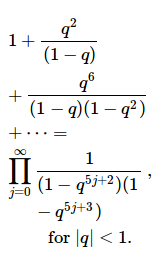
\includegraphics[width=.45 \textwidth]{linebreaking.png}
\end{center}

\end{minipage}


An interface will allow the user to navigate these responsive equations, expanding 
and contracting them as fits their needs and screen real estate. A simple 
demonstration, including the example above, is available at 
\href{http://codepen.io/mathjax/full/dgJHx}{codepen.io/mathjax/full/dgJHx }. 


\section{Team background}

\subsection{The team}

Volker Sorge, Senior Lecturer (Associate Professor) at the University of 
Birmingham, UK, has been working on semantic enrichment and accessibility of 
mathematical documents with his research group for 10 years. He integrated 
accessibility solutions in the context of the European Digital Mathematics 
Library and developed and implemented the mathematics component for ChromeVox 
while at Google, Inc., Mountain View, CA.

The MathJax team consists of Davide Cervone, Christian Perfect, and Peter 
Krautzberger. Davide Cervone, professor at Union College, NY, is MathJax's 
creator and lead developer. He has  pioneered the use of JavaScript for 
mathematical layout since 2004. He also works on WeBWorK, an open-source online 
homework system for math and sciences courses.

Peter Krautzberger is an independent consultant in Bonn, Germany, managing the 
MathJax project. He joined MathJax in 2012 after completing a DFG-funded postdoc 
at the University of Michigan, Ann Arbor. He is an invited expert at the W3C 
Digital Publishing Working Group where he leads the STEM task force. Christian 
Perfect joined MathJax in 2014. He is also the lead developer of the open-source 
assessment system NUMBAS and will not be directly involved in this project.

In short, our team has extensive expertise in the fields of math display, 
processing, and accessibility and a proven track record of producing 
production-ready results combined with an ease of use that enables the widest 
possible audience. 

\subsection{Partners and Collaborators}

MathJax's growing network of collaborators in education, research, and industry 
will provide us with feedback during the project. For example,
\begin{inparaenum}[(a)]
\item we work closely with the \href{http://www.mathjax.org/sponsors/}{MathJax 
sponsors},
\item we have worked with the \href{http://readium.org/}{Readium Foundation} on 
MathML support in their 
epub3 SDK, and 
\item we have good relations with the teams at 
\href{http://hypothes.is/}{Hypothes.is}, \href{http://ipython.org/}{IPython}, 
and \href{http://www.sagemath.org/}{Sage},
\end{inparaenum}
all of whom are interested in better semantics.

\section{Deliverables}

\subsection{Semantic enrichment}

We will develop a JavaScript application that will process MathML, \TeX/\LaTeX, 
and Asciimath to generate MathML with embedded semantic information. This 
information will be generated from heuristics that analyze the MathML, 
identifying its structure, subexpressions, and subject area. 

\subsection{Accessibility tool}

Using this enrichment, we will develop an application to generate speech 
strings as well as navigational information and embed these into MathJax output. 
This will allow accessibility tools to access and navigate the expressions for 
voicing, synchronized highlighting, and other modern accessibility methods. 

\subsection{Responsive equations}

Using the enrichment, we will develop an application to provide a novel way of 
rendering mathematics on small screens by re-arranging and collapsing equations 
meaningfully with a user interface for exploration.

\section{Budget justification}

Our proposal requests funding for a small team that has an excellent track 
record in leading the MathJax project and making math accessible on the web. 
The proposed funds will support these established researchers/developers 
to focus on the complex problems in this proposal. 


\section{Other sources}

The MathJax Consortium and its sponsors support the regular MathJax maintenance 
and development. These resources are not available to support the work outlined 
in this proposal. However, the MathJax Consortium will support travel to 
appropriate conferences and workshops to disseminate the results of the 
research.

% \section{References}
% 
% 
% Kra13: mathml forges on
% 
% Soiffer: http://www.cs.berkeley.edu/~fateman/temp/kajler-soiffer.pdf A survey 
% of 
% user interfaces for computer algebra systems N Kajler, N Soiffer"
% 
% also: http://www.eecs.berkeley.edu/Pubs/TechRpts/1991/6400.html

\end{document}
